\question[10] En la tabla siguiente tabla, anota si cada cantidad aumenta, disminuye o permanece igual.

\begin{table}[H]
    \centering
    \begin{tabular}{|l|l|l|l|l|l|}
        \hline
        Movimiento del patinador &                                               & Energía potencial & Energía cinética & Velocidad & Energía total \\
        \hline
        Subiendo por la pista    & 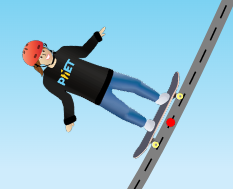
\includegraphics[width=100pt]{../images/up}   &                   &                  &           &               \\
        \hline
        Bajando por la pista     & 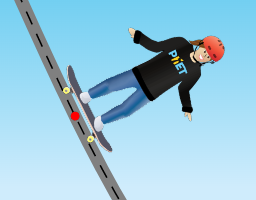
\includegraphics[width=100pt]{../images/down} &                   &                  &           &               \\
        \hline
    \end{tabular}
    \label{tab:upordown}
\end{table}